\documentclass{article}
\setlength{\oddsidemargin}{0.25 in}
\setlength{\evensidemargin}{-0.25 in}
\setlength{\topmargin}{-0.6 in}
\setlength{\textwidth}{6.5 in}
\setlength{\textheight}{8.5 in}
\setlength{\headsep}{0.75 in}
\setlength{\parindent}{0 in}
\setlength{\parskip}{0.1 in}

\usepackage{amsmath,amsfonts,graphicx}
\usepackage{hyperref}
\usepackage{enumitem}
\usepackage{bbm}

\newcounter{lecnum}
\renewcommand{\thepage}{\thelecnum-\arabic{page}}
\renewcommand{\thesection}{\thelecnum.\arabic{section}}
\renewcommand{\theequation}{\thelecnum.\arabic{equation}}
\renewcommand{\thefigure}{\thelecnum.\arabic{figure}}
\renewcommand{\thetable}{\thelecnum.\arabic{table}}

%
% The following macro is used to generate the header.
%
\newcommand{\lecture}[4]{
   \pagestyle{myheadings}
   \thispagestyle{plain}
   \newpage
   \setcounter{lecnum}{#1}
   \setcounter{page}{1}
   \noindent
   \begin{center}
   \framebox{
      \vbox{\vspace{2mm}
    \hbox to 6.28in { {\bf CS 768: Learning With Graphs
        \hfill Autumn 2020-2021} }
       \vspace{4mm}
       \hbox to 6.28in { {\Large \hfill Lecture #1: #2  \hfill} }
       \vspace{2mm}
       \hbox to 6.28in { {\it Instructor: Prof. Abir De \hfill Scribe: #4} }
      \vspace{2mm}}
   }
   \end{center}
   \markboth{Lecture #1: #2}{Lecture #1: #2}
}

%Use this command for a figure; it puts a figure in wherever you want it.
%usage: \fig{NUMBER}{SPACE-IN-INCHES}{CAPTION}
\newcommand{\fig}[3]{
            \vspace{#2}
            \begin{center}
            Figure \thelecnum.#1:~#3
            \end{center}
    }
% Use these for theorems, lemmas, proofs, etc.
\newtheorem{theorem}{Theorem}[lecnum]
\newtheorem{lemma}[theorem]{Lemma}
\newtheorem{proposition}[theorem]{Proposition}
\newtheorem{claim}[theorem]{Claim}
\newtheorem{corollary}[theorem]{Corollary}
\newtheorem{definition}[theorem]{Definition}
\newenvironment{proof}{{\bf Proof:}}{\hfill\rule{2mm}{2mm}}

% **** IF YOU WANT TO DEFINE ADDITIONAL MACROS FOR YOURSELF, PUT THEM HERE:
\newcommand{\Sim}{\text{sim}}

\begin{document}

\lecture{8}{Theoretical Justification of Link Prediction Heuristic }{}{Pintu Kumar, Prantik Chakraborty}
Let $G$ be the orignal graph and $]\hat{G}$ be a graph generated by some link prediction algorithm. Then we want to see a measure of $\Delta(\hat{G},G)$.

\section{Generative Model of $G$}
\begin{itemize}
    \item Build a hyper sphere of volume 1 in the space $\mathbb{R}^d$.
    \item Distribute all the nodes within the sphere uniformly at random.
    \item Set $(u,v)\in E$ if $d_{uv}<r$.
\end{itemize}

\section{Oracle Algorithm A*}
Suppose a Link prediction algorithm $A^*$ knows distance between any pair of nodes. Then sorting edge in basis of $d_{uv}$ gives a algorithm with average precision 1.\\
Let A be any other LP algorithm, If the ranked list given by A is close to the ranked list generated by $A^*$ then we can say $G$ is close to $\hat{G}$.
\\ This is difficult to prove so we prove $d_{min}\approx d_{uv}$, where $u,v$ has highest LP score. This is similar to proving $||d_{min}-d_{uv}||<\epsilon$ with high probability. 
\subsection{Key Points}
\begin{enumerate}
    \item An oracle algorithm which has access to the latent distance between the nodes u and v
    \item In practice the link prediction algorithm does not have access to the  latent distance between the nodes u and v. It can only detect the absence or presence of an edge
    \item There is a generative process using which the graphs are created 
\end{enumerate}

\section{Approach}
\textbf{Main idea:} We assume we can approximate the latent distance between u and v from the graph and the create a ranked list 

\textbf{To prove:} Adamic-Adar and Common-Neighbor can give a reasonable approximate for the latent distance between u and v. The ranked list given by the oracle algorithm and the Adamic-Adar/Common-Neighbor would be roughly same.
\section{Common Neighbours}
Let \mathcal{G}=$\{V,E\}$ be a graph and $N(u)$ denote set of neigbours of $u\in V$. Then for $u,v\in V$
\begin{equation} \label{eq1}
\begin{split}
CN(u,v) & = |N(u)\cap N(v)|\\
& =\sum_{w\in V} |\mathbbm{1}\{w\in N(u)\cap N(v)\}|
\end{split}
\end{equation}
In order to find notation of common neighbours in generated model, calculate $\mathbb{E}[CN(u,v)]$\\
$\mathbb{E}[CN(u,v)]=\sum_{w\in V}\mathbb{P}(w\in N(u)\cap N(v))$.\\ To calculate the probability inside summation, we first calculate $\mathbb{P}(w\in N(u)\cap N(v)|d_{uv})$ .
\begin{equation} \label{eq1}
\begin{split}
\mathbb{P}(w\in N(u)\cap N(v)|d_{uv}) &=\mathbb{P}(u-v-w|d_{uv}\\
&= \int_{d_{uw},d_{wv}}\mathbb{P}(u-w|d_{uw}).\mathbb{P}(w-v|d_{wv}).\mathbb{P}(d_{uw},d_{wv}|d_{uv})\\
&=A(r,d_{uv})
\end{split}
\end{equation}
Here $u-v$ means edge exist between nodes $u$ and $v$. See \ref{fig1} for $A(r,d_{uv})$\\

\begin{figure}[htbp]
\centering
\fbox{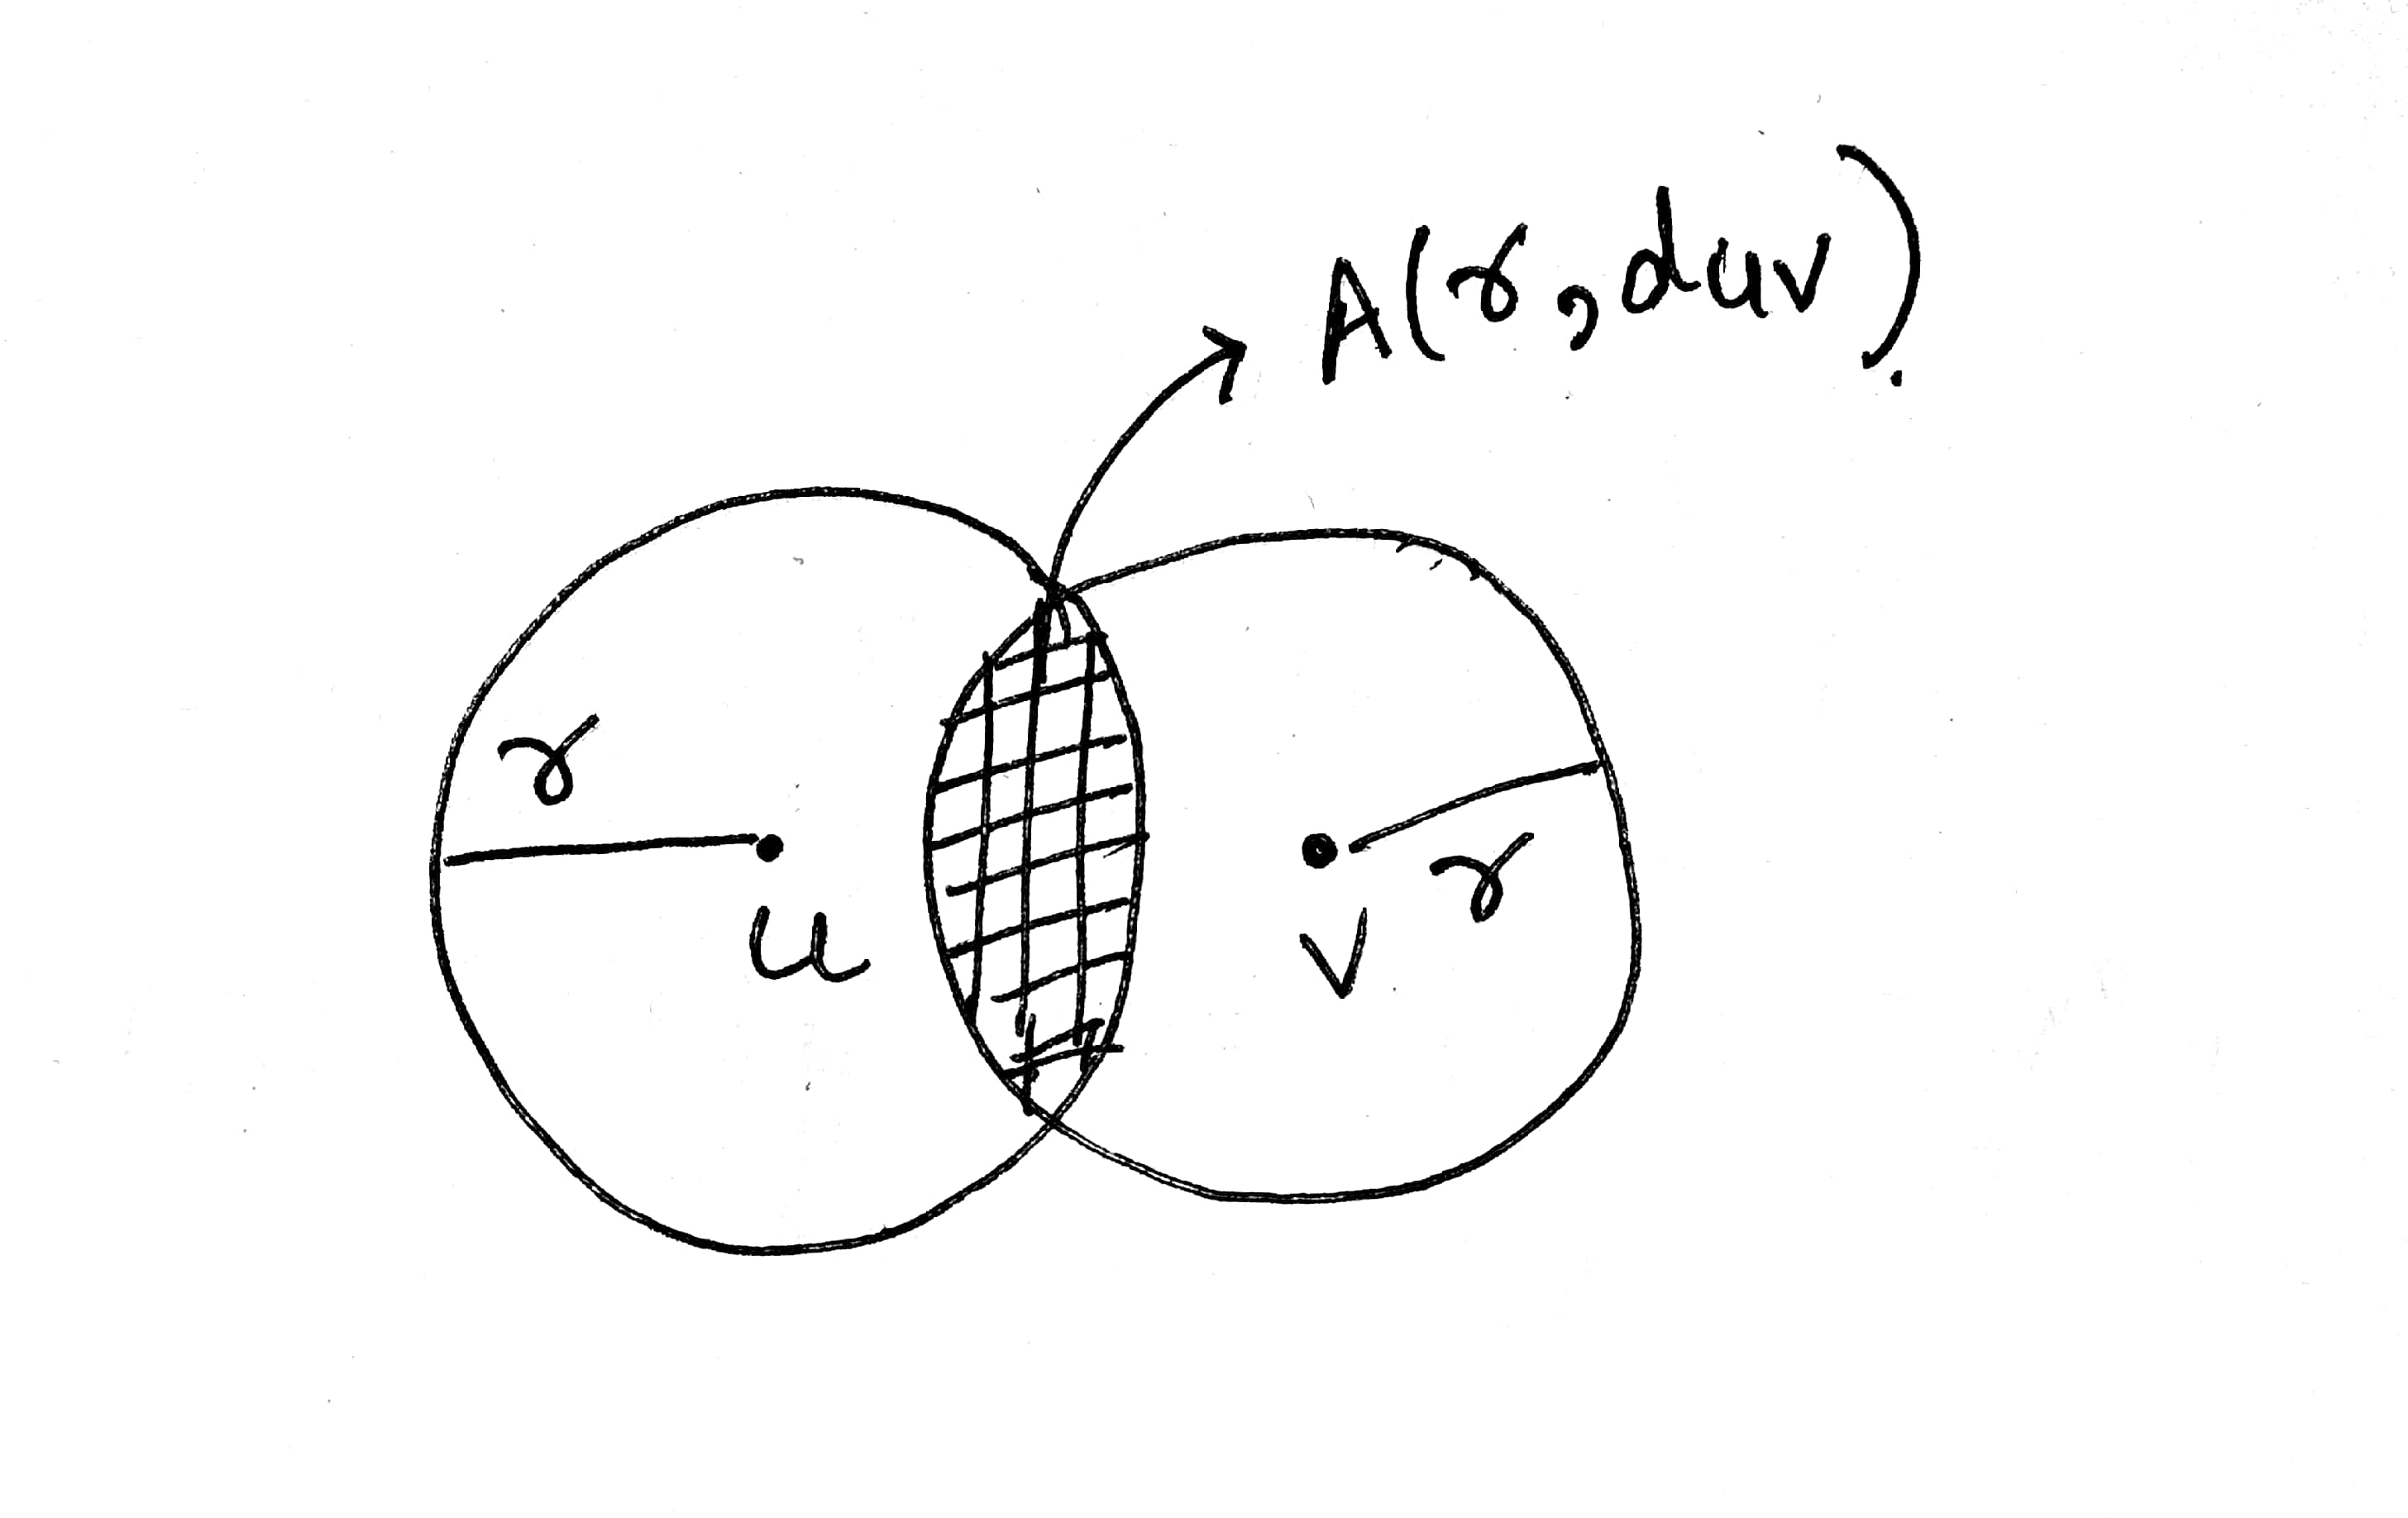
\includegraphics[width=0.8 \linewidth]{pic1.jpg}}
    \caption{Pictorial representation of $A(r,d_{uv})$}
    \label{fig1}
    \end{figure}
Then
\begin{equation} \label{eq3}
\begin{split}
\mathbb{E}[CN(u,v)]&=\sum_{w\in V}\int A(r,d_{uv}).\mathbb{P}(d_{uv})\\
&=|V|\int A(r,d_{uv}).\mathbb{P}(d_{uv})
\end{split}
\end{equation}
This is difficult to compute so variance and expectation of $\mathbbm{1}(w\in N(u)\cap N(v)|d_{uv})$ is used for the proof. Let $X_w$ denote $\mathbbm{1}(w\in N(u)\cap N(v)|d_{uv})$. Then concentration inequality gives. 
\begin{equation} \label{eq4}
\begin{split}
\mathbb{P}(|\sum_{w \in V}\frac{X_w}{|V|}-\mathbb{E}[X_w]|>\epsilon)\leq 2\delta, 
\end{split}
\end{equation}
where 
\begin{equation}
\epsilon =\sqrt{\frac{2Var(X_w).log(2/\delta)}{|V|}}+\frac{3.5log(2/\delta)}{3(|V|-1|)}
\end{equation}
Using inequality \ref{eq4} we show that distance $d_{uv}$ between the node $u$ and $v$ corresponds to the ones giving highest common neighbours score is close to the least possible distance $d_{min}$ (corresponding to $A^*$)
\\~\\
Rather than showing $d_{uv}\approx d_{min}$, we show $A(r,d_{uv})\approx A(r,d_{min})$. Showing this implies $d_{uv}\approx d_{min}$ asymptotically with size of graph.
\
\begin{equation} \label{eq6}
\begin{split}
\mathbb{E}[X_w] &=A(r,d_{uv})\\
&=\frac{2\pi^{\frac{D-1}{2}}r^D}{\Gamma({(D-1)/2)}}\int^{cos^-1(\frac{d_{uv}}{2r})}_0sin^D(t)dt 
\end{split}
\end{equation}\\~\\
A bound on $A(r,d_{uv})$ is given by, 
\begin{equation} \label{eq7}
\begin{split}
\left (1-\frac{d_{uv}}{2r}\right)^D*v(r)\leq A(r,d_{uv})\leq \left(1-\left(\frac{d_{uv}}{2r}\right)^2\right)^\frac{D}{2}*v(r)
\end{split}
\end{equation}\\~\\

Let us define few notation 
\begin{equation}
\epsilon_0 =\sqrt{\frac{2Var(X_w^*).log(2/\delta)}{|V|}}+\frac{3.5log(2/\delta)}{3(|V|-1|)}
\end{equation}
$X_w^*:$ Optimum given by $A^*$

\begin{equation}
\epsilon_m =\sqrt{\frac{2Var(X_w^{CN}).log(2/\delta)}{|V|}}+\frac{3.5log(2/\delta)}{3(|V|-1|)}
\end{equation}
$X_w^{CN}:$ Optimum given by common neighbours.
Then following inequality can be obtained,
\begin{equation}
\mathbb{P}(A(r,d_{uv})>A(r,d_{min})-\epsilon_0-\epsilon_m)\geq 1-2\delta
\end{equation}
Here $d_{uv}$ is the distance between nodes $u$ and $v$ which gives best score for common neighbours, $d_{,min}$ is the distance between nodes $u^*$ and $v^*$ which gives best score for $A^*$, 
\end{document}